\section{Naive Implementation of the Verification Method}
\label{naive}
In this chapter, we show how the algorithm in \ref{verificationalgorithm} can be implemented. The implementation is naïve, in that it strictly follows the mathematical concepts. Finally, we identify the main drawbacks of this naïve implementation and suggest an improved implementation.

\paragraph{Notations}
In this chapter, we use the terms \e{concretizations} and \e{potential concretizations}. The reason for this is that there is no straigh-forward way to go from a set of views to a corresponding set of concretizations. In order to find the concretizations, we generate all of the \e{potential} concretizations, i.e. any extension of a view already in the set with any symbol in the alphabet. Maintaining a set $V_k$ of views of size at most $k$, a view $v\in V_k$ may be extended with a symbol on one or more of its channels, yielding the potential concretization $con$. We say that $con$ is \e{accepted}, if all the views of $con$ of size up top $k$ are in $V_k$, otherwise, $con$ is \e{refuted}. Note that a concretization may be refuted in one iteration but accepted in another, as the set of views $V_k$ may grow to include a larger set of views. We say that the an accepted concretization $con$ is \e{reached} from the view $v$.

\subsection{Naïve implementation}
A naïve way of generating configurations would be to perform the described operations in such a way that they correspond exactly to the mathematical notations described in section \ref{alphagamma}. This is possible to do, as most programming languages have built-in datastructures that support set operations and tuples.

In this naive approach, each configuration is uniquely stored in a \e{set} $V_k$. For each element \e{c} of the set $V_k$, the concretization, post-image and abstraction functions are  ppliedin that sequence, until $V_k$ reaches a \e{fix-point}, i.e. continuing the process does not result in any more configurations being found. Assuming that a set of channel symbols and a set of rules \e{R} describing the transitions are known, the algorithm does the following:


\begin{enumerate}
\item
\textbf{Concretization function}:

Generate a set $\gamma_k^{k+1}$: For each configuration \e{c} $\in$ $V_k$, generate all potential concretizations \e{con}. For any such potential concretization \e{con}, remove those for which $\alpha_k(c')$ $\not\subseteq$ $V_k$.

\item
\textbf{Post-image}:

Generate the set $post(\gamma(V_k))$: For every \e{con} $\in$ $\gamma(V_k)$, \e{r} $\in$ $\delta$, compute $\delta(con)$.

\item
\textbf{Abstraction Function}:

Generate $Apost(V_k)$: For each element \e{p} $\in$ $post(\gamma(V_k))$, compute the set $V'$ of views of size at most \e{k}. If \e{V'} $\cup$ $V_k$ = $V_k$, a fixpoint has been reached, otherwise repeat the process with $V_k$ := $V_k$ $\cup$ $V'$.
\end{enumerate}


\subsection{Improving the Implementation}
Evaluating the procedure described above, we find that the bottle-neck lies the concretization function. In order to find all the concretizations of the set $V_k$, it first creates all potential concretizations of the set $V_k$, by testing all extensions of the views $v \in V_k$, i.e. all combinations of channel evaluations where at least one of the channels is of a larger size than in \e{v}. For each of these potential concretizations, all its views are created in order to determine whether the concretization should be accepted or not.

Although this method is correct, there is significant overlap of concretizations being considered; it is often possible to create the same concretization \e{con} in several ways, and each time the abstract post-image must be calculated. We will show that all concretizations can be found, while considering only a subset of the potential concretizations. Furthermore, it is possible to determine whether a concretization should be accepted or not, examining only a subset of its views. 

\paragraph{Simplified Subword Relation}
Using the fact that the verification algorithm is recursive, ending first when no new configurations can be found, we can re-define the subword relation such that not all views are created at a certain time, but still guaranteeing that all views are found eventually.
We redefine the subword relation in section \ref{words}, such that a word $w' \subword w = a_1a_2\ldots a_n$ if $w' = a_ia_{i+1}\ldots a_j$ for some $0 \leq i \leq n$, $0 \leq j \leq n$. As an example, if \e{w}=$abc$, then the set of subwords of \e{w} is \e{abc, ab, bc, a, b, c, $\varepsilon$}. 

\begin{proof}
Consider a subword of $w = a_1a_2\ldots a_n$ that is a subword according to the original definition of the subword relation, but not by the simplified subword relation, $w' = a_ia_{i+1}\ldots a_ja_la_{l+1}\ldots a_m$, $l > j+1$. If a view $v'$ with the word $w'$ on one of its channels should be accepted, then the set $V_k$ of views necessarily also contains views $v'_1$, $v'_2$, \ldots with the words $a_ia_{i+1}\ldots a_j$, $a_ia_{i+1}\ldots a_ja_l$, $a_ia_{i+1}\ldots a_ja_la_{l+1}\ldots a_{m-1}$ on the channel respectively.

The view $v'_1$ with the word $a_ia_{i+1}\ldots a_j$ would be created with the simplified subword relation, as it is an unbroken sequence of messages. Then the view $v'_2$ with the word $a_ia_{i+1}\ldots a_ja_l$ is a potential concretization of $v'_1$, which would be accepted. The view $v'_3$ with the word $a_ia_{i+1}\ldots a_ja_la_{l+1}$ on the channel is in turn a potential concretization of $v'_2$, which would again be accepted. Continuing in this way, the view with the word $w'$ on the channel will eventually be created and accepted.
\end{proof}

\paragraph{Reducing the number of Concretizations.}
Given a configuration \e{c}, with channel evaluations $\xi$ such that $size(c) \leq k$, a potential concretization of \e{c} is any configuration \e{con} such that \e{con} can be created from \e{c} by appending at least one message to at least one of the channels of \e{c}.
%This is a large number of potential configurations, for which it would be desireable to consider only a subset, while still ensuring that all valid concretizations are eventually found.

Let \e{con} be a concretization reached from \e{v}, where $n$ channels have been extended by a symbol. If such a potential concretization is accepted, any view $v'$ where $n'<n$ channels have been modified in a similar way will also be a valid concretization, since $v' \subword v$. Therefore, \e{con} will eventually be considered also when only one channel is extended in each iteration, but $n$ iterations are required in order to reach it.

This reduces the number of potential concretizations being inspected in each iteration significantly. If we let $s$ denote the size of the alphabet, $t$ the number of channels and $n$ = $size(V_k)$ in a certain iteration we can create upper limits on the number of potential concretizations that are considered. In the naïve version, a potential concretization is created for each combination of symbols $s$ that can be added to a channel (up to $s^k$ combinations), each combination of such extensions on the $t$ different channels. As this must be done for each of the $n$ existing views, the result is a worst case of $O(n*(s^k)^t)$ potential concretizations that may be considered in a single iteration. Using the suggested abstraction, the number of potential concretizations is reduced such that each of the $n$ views is extended with at most 1 symbol on each of its channels, resulting in a worst case of $O(n*s*t)$ potential concretizations.

\paragraph{Reducing the number of views.}
Another limitation of the naïve approach is that in order to determine wether a potential concretization should be refuted or accepted, as a potential concretization is accepted only if all its views are already in the set $V_k$. If potential concretizations are generated as suggested above, the number of views that need be created can be considerably reduced, using the fact that the potential concretization differs from some already existing view by a single symbol on a single channel.
Suppose we want to determine whether a potential concretization \e{con}, genereated from a view $v$ should be accepted or refuted. We know that $con$ has been genereated from $v$ by adding a single symbol $m$ on one of the channels of $v$, whereas the state of $con$ and $v$ are the same, as is the content of the other channels.

\begin{lemma}
Say $con = (s, w_1, \ldots, w_n)$ was created by extending some view $v = (s, w'_1, \ldots, w'_n) \in V_k$ by adding a single message to a single channel such that $w_p = w'_p \bullet m$ for some $p\leq m$ and $w_i = w'_i$ for all $i \neq p$. Then, if $w_p = m_1, m_2 \ldots m$, it suffices to check whether there is a view $v' = (s, w_1, \ldots, w_n) \in V_k$ such that $w_p = m_2\ldots m$, in order to determine if $con$ can be accepted or not.
\end{lemma}

\begin{proof}
Using the simplified subword relation, the views of $con$ either contain the new symbol $m$ in the word $w_p$, or they do not. Any view of $con$ not containing the symbol $m$ in $w_p$ is also a view of $v$, and must exist in $V_k$. Any view containing $m$ in the word $w_p$ does so with $m$ as its last symbol, i.e. there is a prefix of size at most $k$ followed by the message $m$. Any such word is a subword of the largest possible view containing the message $m$, i.e. $m_2\ldots m$.

\end{proof}


\subparagraph{Example.} Suppose we want to determine whether the potential concretization \e{con} = $\conf{s, abc, de}$ created from the view $v = (s, ab, de)$ is an element of $V_2$. It is then sufficient to check that $v'$ = $\conf{S,bc,de}$ is an element of $V_k$.

\newpage
\section{Improved Implementation}

Using the results of the last chapter, the computational complexity of the verifier is greatly reduced, but there are yet several ways to optimize the procedure. The bottle-neck with the procedure at its current state is the choice of a \e{Set} as lone data structure to store configurations. We expect the number of configurations to grow rather large, due to state-space explotion which cannot be avoided automatically (in certain cases, it could be reduced by further abstraction of the model under testing or by removing unnecessary redundancy in the model). Assuming the Set is ordered, inserting an element to the set and finding an element in the set is done in \e{O(log n)} where \e{n} is the number of elements in the set. As a consequence, the function \e{alpha} which determines whether the views of a certain configuration are in the set has complexity $O(p \cdot log n)$ where \e{p} = $|\alpha_k(c)$. We observe that by definition, a view (and a configuration) is of type \e{(S $\times$ $\xi$)}. For any configuration \e{c} = $\conf{s}{\xi}$, it's views will be of the type $\conf{s}{\xi'}$, i.e., the configuration and its views have identical control-parts. It is therefore reasonable to divide the single \e{Set} into a Set of \e{Set}s, where each \e{Set} corresponds to a specific control-state. With such a division, it is sufficient to check whether the views of a configuration reside in the \e{Set} that corresponds to its control-state.

In a best-case scenario, there would be an equal number of configurations for every state in the system. The complexity of checking whether $\alpha_k(c)$ $\in$ $V$ is reduced to $O(p \cdot log (n/s))$ where \e{s} denotes the number of states in the system. The gains of these modifications in terms of computational complexity is difficult to determine, as the number of configurations with a certain control-state are not necessarily well-distributed, but we anticipate that the gains in many cases will be close to the best case scenario.
\subsection{Control-State Partitioning}
Above it was suggested that the set V could be divided into several sets, distinguished by control-states. The number of control-states in a system is finite and unique; For a system with \e{n} processes, the number of states is $\prod\limits_{i=1}^n|p_i|$. This makes it possible to partition the set of configurations into several smaller disjoint sets, such that all configurations in a set have equal control-state. These sets can be stored in a hashmap indexed by control-state.

%\begin{figure}
%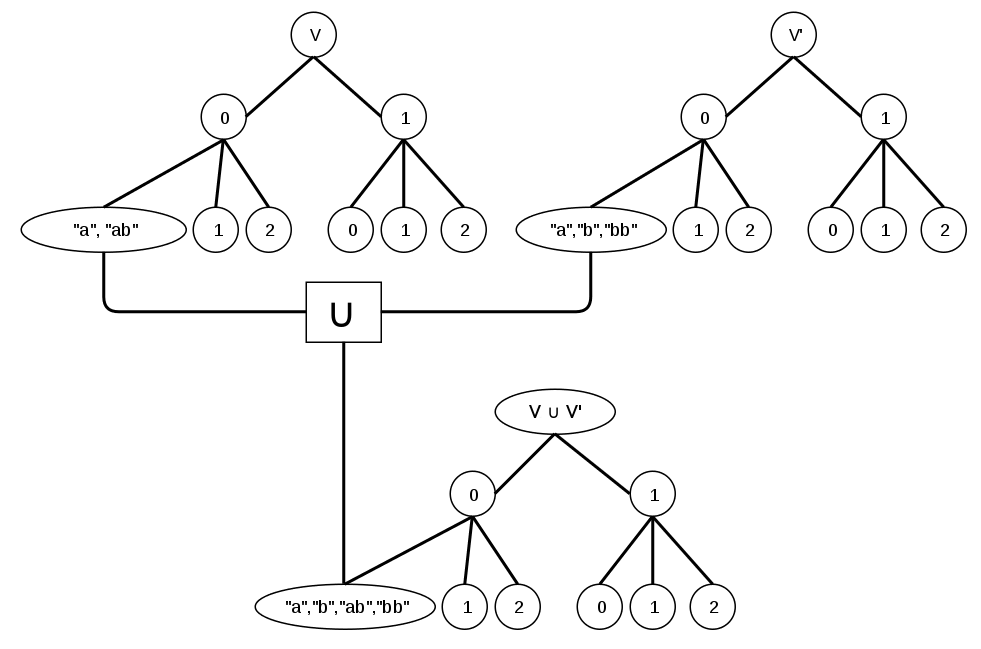
\includegraphics[width=400pt] {bilder/triemerge.png}
%\caption{This picture shows the union of two tries. In this case, there are two processes, the first of which has two states (0 and 1) and the second has three states (0,1 and 2). The union of the trie is the union of their leaves. In the picture, the content of the leaves (0,0) in both threes is made explicit.}
%\label{triemerge}
%\end{figure}


\subsection{Advantages of Partitioning}
Using this partitioning, each node in the hashmap is a \e{Set} with equal-state configurations, addressed by the common control-state. Compared to the previous solution, this leads to a speed-up when inserting, retrieving and looking for the existence of elements in the sets, as the size of the sets will be smaller than before. Retrieving and inserting nodes into the hashmap is done in constant time in practice (the number of elements will be static, avoiding the need of resizing the hashmap).

Having partitioned the configurations, consider the act of applying a rule in order to create a new configuration. Recall that any rule has a state-predicate, a channel-predicate, a state-event and a channel-event. If the predicates are fulfilled, a new configuration can be created by applying the events to the current configuration.

By organizing the set of \e{rules} or transitions in a similar way in a hashmap of rules, we can ensure that the state-predicate is fulfilled without specifically testing for it. A state-predicate is a (possible empty) predicate on the states of the processes in the system, requiring that one or more processes are in a specific state. It is therefore possible to generate a static hashmap of rules, addressed again by control-states.

Considering a transition $t_2$ with no requirements on any processes, the state-predicate will be fulfilled by any configuration, thus a corresponding rule is created in every node of the tree. Consider then instead a transition $t_2$ with requirements on all the processes in the system, i.e. there is only one valid control-state. Such a transition corresponds to a single rule in the node addressed by that control-state. Last, consider a transition $t_3$ with requirements on a true subset of the processes in the system, then the transition can be taken from a number of control-states. These control states can be generated, and the transition will correspond to a set of rules in the nodes corresponding to those control-states.

\paragraph{Example.} Consider yet again the alternating bit protocol, as described in \ref{abpobserver}. The system has three processes \e{Sender}, \e{Receiver} and \e{Observer} with 4, 4 and 3 states respectively. Consider then the transition with the predicates that the sender is in state 3, the observer in state 3 and they may take the synchronized transition with the action \e{Snd} to states 4 and 2 respectively. This transition has no requirements on the receiver, thus it corresponds to four rules, (3,1,3)->(4,1,2), (3,2,3)->(4,2,2), (3,3,3)->(4,3,2), (3,4,3)->(4,4,2). These rules are inserted in the nodes (3,1,3), (3,2,3), (3,3,3) and (3,4,3).

There is a small one-time cost of creating the rule tree, but after creation, it is highly effective. The division by itself ensures that the state-predicate is fulfilled, if not, we never even attempt to apply the rule to a configuration. We illustrate this in figure \ref{applyrule}

\begin{figure}
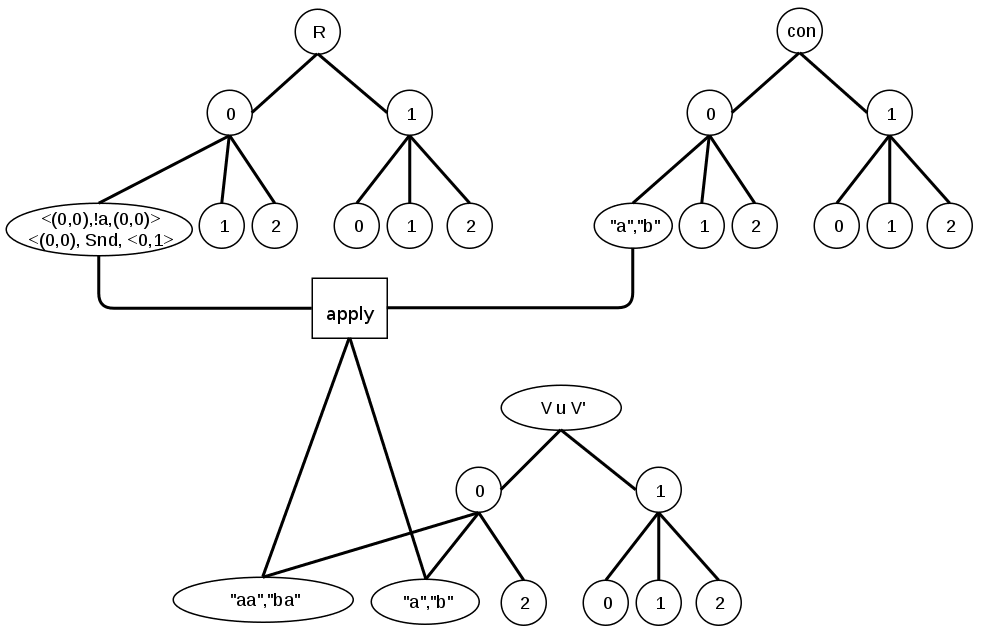
\includegraphics[width=400pt] {bilder/applyrule.png}
\caption{This picture shows the process of applying rules. For each control-state, each rules with that state are applied on each configuration with the same state. This will generate new configurations, not necessarily with the same control-state. This is visualized in a tree, rather than a hashmap, only since hashmap are less intuitive to draw.}
\label{applyrule}
\end{figure}


\begin{algorithm}
  \caption{The verification algorithm from section \ref{alg1} in somewhat higher detail. This version includes }\label{euclid}
  \begin{algorithmic}[1]
    \State \textbf{Gamma (V, Seen):}
    \State \hspace{6 mm} con' := concretizations (V)
    \State \hspace{6 mm} con  := c | c $\in$ con $\land$ c $\notin$ Seen
    \\
    \State \textbf{Step (Con, Rules):}
    \For {state $\in$ nodes(V)}
    \State \hspace{6 mm} S := r(c) | $\forall$ c $\in$ con(state) $\land$ $\forall$ r $\in$ Rules(state)
    \EndFor
    \\
    \State \textbf{Alpha (V, S):}
    \State \hspace{6 mm} V:= V $\cup$ views(C)
    \\
    \State \textbf{Verifier (V, Rules, Bad):}
    \For{\texttt{$True$}}
        \If {$\mathcal{R}_k$ $\cap$ $Bad$ $\neq$ $\emptyset$}
        \State return Unsafe
        \EndIf
        \State V := $\mu Alpha(Step(Gamma(V)))$
        \If {$\gamma_k(V)$ $\cap$ $Bad$ = $\emptyset$}
        \State return Safe
        \EndIf
        \State k := k+1
      \EndFor
\end{algorithmic}
\end{algorithm}

\newpage
\section{Final Implementation}
An efficient algorithm in this context is largely an algorithm that avoids performing unnecessary calculations. This can either be done by avoiding to create unnecessary configurations such as was done with the rule hashmap above or by avoiding re-calculating previously calculated results. The algorithm as described above reproduces its steps each iteration; if a configuration \e{c} can be extended to a concretization \e{con} at any point in the verification process, then \e{con} can and will be created in every following iteration. This includes checking whether \e{$\alpha_k(con) \subset V$}, applying a set of rules to the configuration and then adding all the views of the resulting configurations to the set. Each time the calculations are performed, the result will be duplicates and no new views are added to the system.

We solve this by maintaining another hashmap, \e{seen}, of configurations in parallell, containing exactly those concretization that have been accepted. If a configuration \e{c} can be extended to the concretization \e{con}, then we first check if \e{con} is an element of seen. If it is, we discard \e{con}, otherwise we add \e{con} to \e{seen} and also to the set of concretizations to be evaluated in this iteration.

Yet another source of repetition is the fact that there are multiple ways to create the same channel evaluations. Therefore, after a rule has been applied to a concretization, it may result in a configuration already in the set. Instead of performing the costly $\alpha$-calculation, we first check if the newly created configuration is not in fact a duplicate by checking if it is already in \e{V}. If so, the configuration can again be discarded.

The final algorithm amounts to the following pseudo-code representation:

\subsection{Reachability Analysis}
An important step of the verification process which has yet to be covered is that of performing a reachability analaysis, in order to find bad states, if any such states are reachable and find a minimal bad trace leading up to the bad state. See sections \ref{bad} and \ref{traces} for formal definitions of bad states and traces respectively.

Below, a simple technique of finding a minimal bad trace is presented, accompanied with a proof that the trace is in fact minimal.

\subparagraph{Finding Minimal Traces}
When running the verification, if a bad state is found we want to produce a trace leading up to the bad state. Preferably, this would be a minimal trace that leads to the bad state.

The proposed verification method generates a finite set of reachable states (nodes in this context), but it does not record the available transitions between the nodes (i.e. the edges). It is possible to for each node \e{n} to save all nodes \e{n} from which an edge to \e{n'} exists, and thus build the complete reachability graph of the problem. There exists efficient algorithms to solve such a problem, e.g. \e{dijkstra shortest path}, or even the shortest path between any two nodes, e.g. flow-network techniques. Although these algorithms are efficient, building the complete reachability graph would be costly in terms of memory space, as the number of edges may be much larger than the number of states.


We show that due to the method of iteratively constructing the graph, nodes are created in such a way, that if a node $n_{i}$ created in the \e{i}:th iteration is reached by a node $n_{i-1}$ over an edge $e_{i-1}$, the shortest path from the initial node $n_0$ will necessarily be a path $e_1...e_{i-1}$.

\e{Proof.} This is proven using an induction proof. We hypothesize that, if at the point of creation of $n_i$, choosing the parent node $n_{i-1}$ from which an edge $e_{i-1}$ can be taken $n_i$, the path $e_1..e_{i}$ will be the shortest path to $n_i$ and has length \e{i}. Note that the node $n_{i-1}$ must have been created in the previous iteration; had it been created earlier, the edge $e_i$ could have been taken in a previous iteration, and so $n_{i+1}$ would already be a node in the tree.

The base case is that for any node reachable from $n_0$ over any edge $e_0$, $e_0$ will be the shortest path and has length 1. This is trivially true.

Now suppose a node $n_{i+1}$ is reachable over an edge $e_i$ from a node $n_i$, and the node $n_{i+1}$ is not yet in the system. The induction hypothesis states that the path $e_1...e_i$ is the shortest path leading up to $n_i$. If $e_0..e_{i-1}e_i$ would not be the shortest path to $n_{i+1}$, there would be a path $e'_0..e'_{k-1}$ to another node $n_k$ with k < i from which $n_{i+1}$ can be reached. But any such node would have been created in the \e{k}:th iteration of the algorithm, which would contradict the fact that the node $n_{i+1}$ was not already in the system.

Having shown this, we need only record the information of a single parent of a node, in order to build up a tree from which the shortest path from $n_0$ to any node in the system can efficiently be found.


\subsection{Specification Language}
\label{speclang}
In order for the verification algorithm to be easily used, a specification language is needed in which algorithms can be formally defined. We expect such a specification language to

\begin{itemize}
\item
be expressive enough to express all algorithms that are in the scope of the verification program
\item
be independent of the internal representations of the verifier and to demand as little knowledge of the actual verification process as possible from the user
\item
to be as clear as possible in order to ensure that the model at hand in fact corresponds to the actual algorithm, the way it was intended
\end{itemize}

The specification language used is an adaption of previous works in \cite{mpass}. The language simply uses XML to describe an algorithm. There are minor differences between the specification language used here, with respect to that used in by the MPass verification algorithm, and correspond to different expressivness of the models. More specifically, the MPass verifier allows for joint reception and transmission transitions, i.e. a single transition may read a message from a channel and write a message to a channel at the same time. On the other hand, it does not allow for synchronized transitions, this has therefore been added to the language.

\subsubsection{Example}
We return yet again to the Alternating Bit Protocol to examplify the specification language. Bearing in mind the formal definition in section \ref{CS}, a model needs a set of messages, channels, actions and transitions.

We begin by specifying a new protocol, it's name and that it is operating on FIFO buffers. We then specify a set of messages, a set of channels and a set of actions in a similar manner.

\lstset{language=XML}
\begin{lstlisting}[frame=single]
<protocol name="Alternating Bit Protocol" medium="FIFO>
<messages>
      <message>ack0</message>
      <message>ack1</message>
      <message>mesg0</message>
      <message>mesg1</message>
</messages>

<channels>
      <channel>c1</channel>
      <channel>c2</channel>
</channels>

<actions>
      <action>Rcv</action>
      <action>Snd</action>
</actions>
\end{lstlisting}

We then continue by defining the different processes in the system, i.e. the sender, receiver and observer. Such a process is defined by its states and its transitions. In the specification language, we differentiate between transitions over an action, and transitions that modify a channel. The latter type is called a \e{rule} in the specification language, in order to comply with the names used in the MPass specification language. This should not be confused with the word as used earlier in this section.

\begin{lstlisting}[frame=single]
  <role name="SENDER">
    <states>
      <state type="initial">Q0</state>
      <state>Q1</state>
      <state>Q2</state>
      <state>Q3</state>
    </states>
    <action>
        <current_state>Q0</current_state>
        <type>Snd</type>
        <next_state>Q1</next_state>
    </action>
    <rule>
        <current_state>Q1</current_state>
        <send_message>mesg0</send_message>
        <next_state>Q1</next_state>
        <channel>c1</channel>
    </rule>
\end{lstlisting}

Last, we specify that the processes \texttt{SENDER} and \texttt{OBSERVER}, and  \texttt{RECEIVER} and \texttt{OBSERVER} are to be synchronized over the actions \texttt{Snd} and \texttt{Rcv} respectively.

\begin{lstlisting}[frame=single]
<synchronize>
        <first_role>SENDER</first_role>
        <second_role>OBSERVER</second_role>
        <action>Snd</action>
</synchronize>
<synchronize>
        <first_role>RECEIVER</first_role>
        <second_role>OBSERVER</second_role>
        <action>Rcv</action>
</synchronize>
\end{lstlisting}
